% Module E: Audit-First AI
% INStats Data Can Deceive: Causal Roadmaps with (and without) AI workshop
% August 5, 2026 | Auriane Journet

\documentclass[aspectratio=169]{beamer}

% Theme and packages
\usetheme{metropolis}
\usepackage[utf8]{inputenc}
\usepackage{amsmath, amssymb, mathtools, bm}
\usepackage{graphicx}
\usepackage{booktabs}
\usepackage{lmodern}
\usefonttheme{professionalfonts}
\usepackage{microtype}
\usepackage{xcolor}
\usepackage{hyperref}
\hypersetup{hidelinks}
\usepackage[absolute,overlay]{textpos}
\usepackage{tikz}
\usetikzlibrary{positioning,arrows.meta,shapes.geometric,calc}
\usepackage[numbers]{natbib}

\title[Auditing AI Output]{Auditing AI Output}
\subtitle{Data Can Deceive: Causal Roadmaps with (and without) AI}
\author{Auriane Journet}
\institute{Module E: Audit-First AI}
\date{August 5, 2026 \quad $\cdot$ \quad 2:20--2:45 ET}

\definecolor{accent}{HTML}{4A9EFF}
\definecolor{brick}{HTML}{C0392B}
\definecolor{good}{HTML}{27AE60}
\definecolor{inkdark}{HTML}{23373B}
\setbeamercolor{structure}{fg=accent}
\setbeamercolor{background canvas}{bg=white}
\metroset{progressbar=frametitle,block=fill}
\setbeamertemplate{navigation symbols}{}
\setbeamertemplate{footline}{}

% TikZ styles for the mini-DAGs.  Node positions are held constant across
% all graphs so that only the arrow directions change.
\tikzset{
  var/.style={circle, draw=black!70, thick, minimum size=8mm, inner sep=1pt, font=\small},
  tx/.style ={circle, draw=accent, fill=accent!12, very thick, minimum size=8mm, inner sep=1pt, font=\small},
  outc/.style={circle, draw=black!70, thick, minimum size=8mm, inner sep=1pt, font=\small},
  edge/.style={-{Stealth[length=2.2mm]}, thick},
  badj/.style={-{Stealth[length=2.2mm]}, thick, brick},
  lab/.style ={draw=black!55, rounded corners, thick, minimum height=6mm, inner sep=3pt, font=\scriptsize, align=center},
  labtx/.style={draw=accent, fill=accent!12, rounded corners, very thick, minimum height=6mm, inner sep=3pt, font=\scriptsize, align=center},
  un/.style  ={circle, draw=black!45, dashed, thick, minimum size=7mm, inner sep=1pt, font=\scriptsize},
  cond/.style={draw=brick, dash pattern=on 2pt off 1.5pt, very thick, rounded corners, minimum height=6mm, inner sep=3pt, font=\scriptsize, align=center},
  spur/.style={{Stealth[length=1.8mm]}-{Stealth[length=1.8mm]}, dashed, brick, thick},
}

% Verdict tags (reuse the template palette: good / accent / brick)
\newcommand{\vaccept}{\textcolor{good}{\textbf{ACCEPT}}}
\newcommand{\vcorrect}{\textcolor{accent}{\textbf{CORRECT}}}
\newcommand{\vreject}{\textcolor{brick}{\textbf{REJECT}}}

\begin{document}

% ======================================================================
% Section divider
% ======================================================================
\begin{frame}[plain]
  \centering
  \vfill
  {\usebeamerfont{title}\color{inkdark}\textbf{\Large Auditing AI Output}}\\[0.6em]
  {\color{accent}\normalsize Data Can Deceive \(\cdot\) Causal Roadmaps with (and without) AI}\\[0.9em]
  {\color{inkdark}\small\textbf{Module E}}\\[0.35em]
  {\color{black!55}\small August 5, 2026}\\[0.9em]
  {\color{black!60}\small Auriane Journet}
  \vfill
  \begin{textblock*}{3cm}(11.9cm,0.4cm)
    
\includegraphics[width=2.6cm]{art/InStats_RWL.png}
  \end{textblock*}
\end{frame}

% ======================================================================
% Slide 2 - Framing
% ======================================================================
\begin{frame}{A Confident Answer Is Not a Correct One}
  \small
  \begin{itemize}
    \item The model will \textbf{not} tell you when it is wrong; fluency is not validity.
    \item ``Human in the loop'' does \emph{not} mean reviewing the output and nodding.
    \item It means \textbf{auditing each claim} against the evidence that would justify it.
  \end{itemize}
  \vspace{0.8em}

  \begin{block}{Our test case}
    An \textbf{adjustment set} for a \textbf{target-trial protocol} [1]
    --- the list of variables an analysis will control for.
  \end{block}
  \vspace{0.4em}

  \textcolor{accent}{\textbf{Objective:}} turn a confident list of covariates into a set of
  checkable claims.
\end{frame}

% ======================================================================
% Slide 3 - The artifact under audit
% ======================================================================
\begin{frame}{Test Case}
  \small
  \textcolor{accent}{\textbf{Our prompt}}
  \begin{quote}\small
    ``Among adults initiating an SGLT2 inhibitor versus a DPP-4 inhibitor for
    type~2 diabetes, does the SGLT2 inhibitor reduce hospitalization for heart
    failure? List the variables to adjust for so the groups are comparable.''
  \end{quote}

  \textcolor{accent}{\textbf{The model's answer}}
  \begin{quote}\small
    ``Adjust for: age, sex, baseline eGFR, baseline HbA1c, prior heart failure,
    prior MI, baseline diuretic use, HbA1c at 6 months, and change in eGFR on treatment. Adjusting for
    glycemic control and renal response removes any residual imbalance in disease
    severity.''
  \end{quote}

  {\footnotesize\textcolor{accent}{\textbf{Side note:}} models vary and change fast, a
  good answer today can be a bad one tomorrow. The key point is to build the habit of
  auditing a model's answer \emph{regardless} of how confident it sounds.}
\end{frame}

% ======================================================================
% Slide 4 - Activity: first pass
% ======================================================================
\begin{frame}{Step 1: First Pass}
  \small
  \begin{block}{Answer in the chat}
    Read the nine variables suggested by the model. \textbf{Flag any you would question}
    and say why in a few words.
  \end{block}
  \vspace{0.4em}

  \begin{columns}[T]
    \begin{column}{0.5\textwidth}
      \begin{itemize}
        \item age
        \item sex
        \item baseline eGFR
        \item baseline HbA1c
        \item prior heart failure
      \end{itemize}
    \end{column}
    \begin{column}{0.5\textwidth}
      \begin{itemize}
        \item prior MI
        \item baseline diuretic use
        \item HbA1c at 6 months
        \item change in eGFR on treatment
      \end{itemize}
    \end{column}
  \end{columns}
\end{frame}

% ======================================================================
% Slide 5 - The audit
% ======================================================================
\begin{frame}{Step 2: Audit}
  \small
  \begin{itemize}
    \item Baseline timing is \textbf{necessary but not sufficient}: accept a
      covariate only when substantive knowledge and the DAG support a
      common-cause role.
    \item \textcolor{brick}{HbA1c at 6 months} and \textcolor{brick}{on-treatment
      eGFR change} are measured \textbf{after} treatment starts.
    \item They sit on the causal pathway (\textbf{mediators}) and can act as
      \textbf{colliders}.
    \item Adjusting for them \textbf{blocks part of the effect} you want and can
      \textbf{manufacture bias}.
  \end{itemize}
  \vspace{0.5em}
\end{frame}

% ======================================================================
% Slide 6 - Baseline vs post-baseline
% ======================================================================
\begin{frame}{Baseline vs Post-Baseline}
  \small
  \begin{columns}[T]
    \begin{column}{0.46\textwidth}
      \centering
      \textbf{Baseline confounder}\\ {\scriptsize measured \emph{before} time zero}\\[0.9em]
      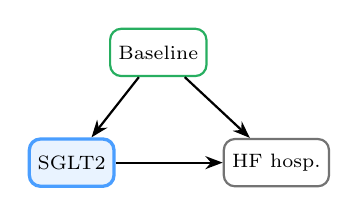
\begin{tikzpicture}
        \node[lab,draw=good] (Z) at (1.1,1.4) {Baseline};
        \node[labtx] (A) at (0,0)   {SGLT2};
        \node[lab]   (Y) at (2.6,0) {HF hosp.};
        \draw[edge] (Z) -- (A);
        \draw[edge] (Z) -- (Y);
        \draw[edge] (A) -- (Y);
      \end{tikzpicture}\\[0.9em]
      \textcolor{good}{\textbf{Adjust}} to close the backdoor.
    \end{column}
    \begin{column}{0.52\textwidth}
      \centering
      \textbf{Post-baseline variable}\\ {\scriptsize HbA1c$_6$ / $\Delta$eGFR, measured \emph{after} time zero}\\[0.9em]
      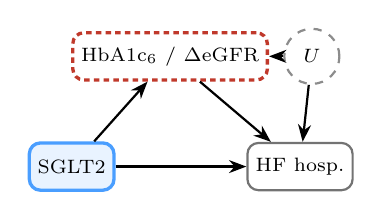
\begin{tikzpicture}
        \node[cond]  (M) at (1.25,1.4) {HbA1c$_6$ / $\Delta$eGFR};
        \node[un]    (U) at (3.05,1.4) {$U$};
        \node[labtx] (A) at (0,0)      {SGLT2};
        \node[lab]   (Y) at (2.9,0)    {HF hosp.};
        \draw[edge] (A) -- (M);
        \draw[edge] (M) -- (Y);
        \draw[edge] (A) -- (Y);
        \draw[edge] (U) -- (M);
        \draw[edge] (U) -- (Y);
      \end{tikzpicture}\\[0.9em]
      \textcolor{brick}{\textbf{Do not adjust}} --- removes the \emph{mediated part} of the total effect \emph{and} opens collider bias via $U$.
    \end{column}
  \end{columns}
  \vspace{0.6em}

  {\footnotesize\textcolor{accent}{\textbf{Assumption:}} the collider
  path needs $U\!\to\!M$ (unmeasured severity affects on-treatment response). Drawing out
  the DAG helps make these assumptions clearer.}
\end{frame}

% ======================================================================
% Slide 7 - Step 3: Decide and Justify
% ======================================================================
\begin{frame}{Step 3: Decide and Justify}
  \small
  \begin{itemize}
    \item Every field gets one of three verdicts: \vaccept\ / \vcorrect\ / \vreject.
    \item Each verdict is \textbf{paired with the evidence} that justifies it (otherwise
      it is just another confident assertion).
    \item For each covariate in your set, answer:
      \begin{itemize}
        \item Was it measured \textbf{before time zero}?
        \item \textbf{Where does it sit on the DAG} (confounder, mediator, collider)?
      \end{itemize}
  \end{itemize}
  \vspace{0.5em}

  \begin{block}{Next step}
    \vaccept\ keep as-is \quad
    \vcorrect\ keep but fix (definition / timing / add a missing one) \quad
    \vreject\ remove
  \end{block}
\end{frame}

% ======================================================================
% Slide 8 - Step 4: Keep an audit log (answer key)
% ======================================================================
\begin{frame}{Step 4: Keep an Audit Log}
  \scriptsize
  \setlength{\tabcolsep}{3pt}
  \renewcommand{\arraystretch}{1.2}
  \begin{tabular}{@{}p{2.5cm} p{1.6cm} l p{5.6cm}@{}}
    \toprule
    \textbf{Variable} & \textbf{Timing} & \textbf{Verdict} & \textbf{Justification} \\
    \midrule
    age, sex & pre-time-zero & \vaccept & Fixed at baseline; affect prescribing and HF risk. \\
    baseline eGFR, HbA1c & pre-time-zero & \vaccept & Indication / severity confounders present before treatment. \\
    prior HF, prior MI & pre-time-zero & \vaccept & Strong confounders of treatment choice and outcome. \\
    baseline diuretic use & pre-time-zero & \vcorrect & Keep, but flag as a \emph{proxy} for HF severity; define the lookback window. \\
    \textcolor{brick}{HbA1c at 6 months} & \textcolor{brick}{post-baseline} & \vreject & Mediator on $A\!\to\!Y$; collider with $U$. Adjusting biases the total effect. \\
    \textcolor{brick}{$\Delta$eGFR on treatment} & \textcolor{brick}{post-baseline} & \vreject & On the causal pathway; conditioning removes the mediated part and opens a collider. \\
    \bottomrule
  \end{tabular}
  \vspace{0.5em}

\end{frame}

% ======================================================================
% Slide 9 - What if I care about the mediator?
% ======================================================================
\begin{frame}{When the Mediator Is the Question}
  \small
  \vaccept\ / \vreject\ assume you want the \textbf{total effect} of treatment.
  For that estimand, ``post-baseline $\Rightarrow$ reject'' is right.
  \vspace{0.6em}

  \begin{block}{Controlling for mediators}
    If the \emph{mediated pathway itself} is your question, how much of the effect
    runs \emph{through} HbA1c or eGFR, that is a \textbf{mediation analysis}. With
    treatment-affected confounding it calls for \textbf{g-methods} (g-computation,
    IPTW, TMLE) [2].
  \end{block}
  \vspace{0.4em}

  {\color{black} Reject the mediator \emph{for a total effect}, and model it deliberately
  when it \emph{is} the target. Do not apply the checklist bluntly.}
\end{frame}

% ======================================================================
% Slide 10 - Transfer task
% ======================================================================
\begin{frame}{Your Turn!}
  \small
  \textbf{Target trial.} Among adults with COPD initiating \textbf{inhaled
  corticosteroids (ICS)} versus a long-acting bronchodilator alone, do ICS reduce
  \textbf{severe exacerbations} over the next year?
  \vspace{0.6em}

  \textbf{Proposed adjustment set:}
  \begin{columns}[T]
    \begin{column}{0.5\textwidth}
      \begin{itemize}
        \item age
        \item prior-year exacerbation count
        \item baseline blood eosinophils
      \end{itemize}
    \end{column}
    \begin{column}{0.5\textwidth}
      \begin{itemize}
        \item smoking
        \item blood eosinophils at 3 months on ICS
      \end{itemize}
    \end{column}
  \end{columns}
  \vspace{0.5em}

  \textcolor{accent}{\textbf{Your task:}} for each variable, draw a DAG and run the audit test
  $\Rightarrow$ \vaccept\ / \vcorrect\ / \vreject.
  \textbf{Anything missing?}
\end{frame}

% ======================================================================
% Slide 11 - Solution
% ======================================================================
\begin{frame}{Solution}
  \scriptsize
  \begin{columns}[T]
    \begin{column}{0.56\textwidth}
      \begin{itemize}
        \item age, prior exacerbations, baseline eosinophils: \vaccept\\
          {\scriptsize pre-time-zero confounders of ICS use and exacerbations}
        \item smoking: \vcorrect\\
          {\scriptsize keep, but define: baseline status / pack-years, before time zero}
        \item eosinophils at 3 months: \vreject\\
          {\scriptsize post-baseline mediator: ICS lowers eosinophils $\to$ fewer exacerbations}
        \item \emph{missing} baseline FEV$_1$: \vcorrect\ (\textbf{add})\\
          {\scriptsize airflow severity confounds both ICS use and exacerbations}
      \end{itemize}
    \end{column}
    \begin{column}{0.44\textwidth}
      \centering
      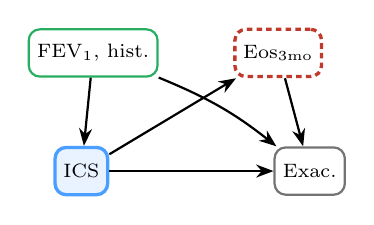
\begin{tikzpicture}[font=\scriptsize]
        \node[lab,draw=good] (Z) at (0.15,1.5) {FEV$_1$, hist.};
        \node[cond]          (M) at (2.5,1.5)  {Eos$_{3\text{mo}}$};
        \node[labtx] (A) at (0,0)   {ICS};
        \node[lab]   (Y) at (2.9,0) {Exac.};
        \draw[edge] (Z) -- (A);
        \draw[edge] (Z) to[bend left=8] (Y);
        \draw[edge] (A) -- (M);
        \draw[edge] (M) -- (Y);
        \draw[edge] (A) -- (Y);
      \end{tikzpicture}\\[0.4em]
      {\scriptsize\textcolor{good}{green = adjust}\ \ \textcolor{brick}{red box = do not}}
    \end{column}
  \end{columns}
  \vspace{0.15em}

\end{frame}

% ======================================================================
% Slide 12 - Takeaways
% ======================================================================
\begin{frame}{Takeaways}
  \small
  \setbeamercolor{enumerate item}{fg=black}
  \begin{block}{Auditing any adjustment set}
    \begin{enumerate}
      \setlength\itemsep{0.35em}
      \item \textbf{Question the model's output}: is each variable measured \emph{before} treatment starts?
      What is a given variable's position on a DAG (confounder, mediator, or collider)?
      \item \textbf{Audit}: \vaccept\ / \vcorrect\ / \vreject\ for each. An omitted confounder
      is a finding too (\vcorrect\ $\to$ add).
      \item \textbf{Justify}
      \item \textbf{Document}
    \end{enumerate}
  \end{block}
  \vspace{0.5em}

  {\color{black} The completed log \emph{is} your causal assumptions made explicit
  and reproducible, as opposed to a black-box list of covariates [2].}
\end{frame}

% ======================================================================
% Slide 13 - Handoff
% ======================================================================
\begin{frame}[standout]
  Audit each claim \textbf{against its evidence}.\\[0.8em]
  Module F carries the corrected roadmap into the Navigator.
\end{frame}

% ======================================================================
% Bibliography
% ======================================================================
\begin{frame}[allowframebreaks]{References}
  \tiny
  \bibliographystyle{plainnat}
  \begin{thebibliography}{9}
    \bibitem{hernan2016target}
    Hern{\'a}n MA, Robins JM.
    \newblock Using big data to emulate a target trial when a randomized trial is not available.
    \newblock \textit{American Journal of Epidemiology}, 183(8):758--764, 2016.

    \bibitem{hernan2020causal}
    Hern{\'a}n MA, Robins JM.
    \newblock \textit{Causal Inference: What If}.
    \newblock Chapman \& Hall/CRC, 2020.

  \end{thebibliography}
\end{frame}

\end{document}
